\documentclass{article}
\usepackage[utf8]{inputenc}
\usepackage{amsmath}
\usepackage{ifsym}
\usepackage{tikz}
\usetikzlibrary{shapes}
\usepackage{cleveref}
\usepackage{tikz}
\usetikzlibrary{positioning, calc}
\usetikzlibrary{trees}
\title{Query Optimization Exercise 8}

\usepackage{amssymb}
\def\roj{\mathbin{\bowtie\mkern-5.8mu\ojoin}}
\usepackage[bottom]{footmisc}

\date{January 2021}

\begin{document}

\maketitle

\section{Exercise 1}
We begin by listing the possible options for ordering with descending ordering Benefit (omitting any orderings with benefit smaller than 1).
\begin{center}
\begin{tabular}{c|c}
Relation & ordering Benefit \\ \hline
$(R_3 \bowtie R_0, R_3 \bowtie R_2)$ & 2 \\
$(R_1 \bowtie R_4, R_1 \bowtie R_0)$ & $\frac{500}{251} \approx 1.992$ \\
$(R_1 \bowtie R_2, R_1 \bowtie R_0)$ & $\frac{5}{3} \approx 1.667$ \\
$(R_0 \bowtie R_3, R_0 \bowtie R_1)$ & $\frac{150}{101} \approx 1.485$ \\
$(R_2 \bowtie R_3, R_2 \bowtie R_1)$ & $\frac{5}{4} = 1.25$ \\
$(R_1 \bowtie R_4, R_1 \bowtie R_2)$ & $\frac{300}{251} \approx 1.195$
\end{tabular}
\end{center}

\begin{tikzpicture}
    \node (L0) {$R_0$};
    \node (L1) [right=of L0] {$R_1$};
    \node (L4) [right=of L1] {$R_4$};
    \node (L3) [below=of L0] {$R_3$};
    \node (L2) [below=of L1] {$R_2$};
    \draw
        (L0) edge (L1)
        (L1) edge (L4)
        (L0) edge (L3)
        (L2) edge (L3)
        (L1) edge (L2);
\end{tikzpicture}

\subsection{Step 1}
\begin{center}

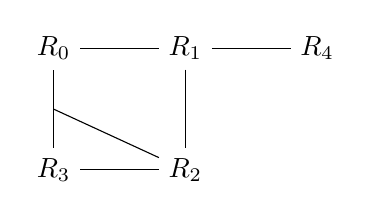
\begin{tikzpicture}
    \node (L0) {$R_0$};
    \node (L1) [right=of L0] {$R_1$};
    \node (L4) [right=of L1] {$R_4$};
    \node (L3) [below=of L0] {$R_3$};
    \node (L2) [below=of L1] {$R_2$};
    \draw
        ($(L0)!0.5!(L3)$) edge (L2) edge (L3) edge (L0)
        (L1) edge (L4)
        (L2) edge (L3)
        (L0) edge (L1)
        (L1) edge (L2);
\end{tikzpicture}
\end{center}
Update of ordering Benefit:
\begin{center}
\begin{tabular}{c|c}
Relation & ordering Benefit \\ \hline
$((R_3 \bowtie R_2) \bowtie R_0, R_0 \bowtie R_1 )$ & $\frac{25}{11}\approx 2.27$ \\
$(R_1 \bowtie R_4, R_1 \bowtie R_0)$ & $\frac{500}{251} \approx 1.992$ \\
$(R_1 \bowtie R_2, R_1 \bowtie R_0)$ & $\frac{5}{3} \approx 1.667$ \\
$(R_0 \bowtie R_3, R_0 \bowtie R_1)$ & $\frac{150}{101} \approx 1.485$ \\
$(R_2 \bowtie R_3, R_2 \bowtie R_1)$ & $\frac{5}{4} = 1.25$ \\
$(R_1 \bowtie R_4, R_1 \bowtie R_2)$ & $\frac{300}{251} \approx 1.195$
\end{tabular}
\end{center}
\subsection{Step 2}

\begin{center}

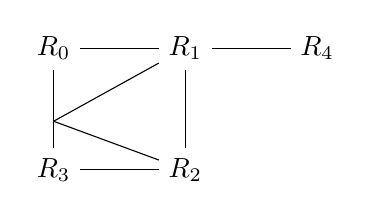
\begin{tikzpicture}
    \node (L0) {$R_0$};
    \node (L1) [right=of L0] {$R_1$};
    \node (L4) [right=of L1] {$R_4$};
    \node (L3) [below=of L0] {$R_3$};
    \node (L2) [below=of L1] {$R_2$};
    \draw
        % ($(L0)!0.5!(L3)$) edge (L2) edge (L3) edge (L0)
        ($(L0)!0.6!(L3)$) edge (L0) edge (L2) edge (L3) edge (L1)
        (L3) edge (L0)
        (L1) edge (L4)
        (L0) edge (L3)
        (L0) edge (L1)
        (L1) edge (L2)
        (L3) edge (L2);

\end{tikzpicture}
\end{center}
\section{Exercise 2}
We assume for this exercise that the right outer join has the same properties regarding associativity as the left outer join.

\begin{center}

\begin{tikzpicture}[level distance=1.5cm,
  level 1/.style={sibling distance=3cm},
  level 2/.style={sibling distance=3cm},
  level 3/.style={sibling distance=3cm},
  level 4/.style={sibling distance=1.5cm}]
  node {$\bowtie_{A.x=B.y}$}
    child {node {$A$}}
    child {node {$\bowtie_{B.x=C.y}$} %first right
      child {node {$B$}} %second left
      child {node {$\bowtie_{-}^{\_\_C.x=E.y}$} %second right
        child{ node{$\bowtie_{C.y=D.x}$} %third left
          child{node {$C$}}%forth left
          child{node {$D$}}%forth right
        }
        child{ node{ {$\bowtie_{E.x = F.y}$}} %third right
          child{node {$E$}}%forth left
          child{node {$F$}}%forth right
            }
      }
    }
\end{tikzpicture}
\end{center}
\begin{center}
\begin{tabular}{c|c}
SES & TES \\ \hline
$\{A,B\}$ & $\{A,B\}$\\
$\{B,C\}$ & $\{B,C,D,E\}$\\
$\{C,E\}$ & $\{C,D,E\}$\\
$\{C,D\}, \{E,F\}$ & $\{C,D\}, \{E,F\}$\\
\end{tabular}
\end{center}

\begin{center}

\begin{tikzpicture}
    \node (LC) {$C$};
    \node (LE) [right=of LC] {$E$};
    \node (LF) [right=of LE] {$F$};
    \node (LD) [below=of LC] {$D$};
    \node (LB) [below=of LE] {$B$};
    \node (LA) [right=of LB] {$A$};
    \draw
        % ($(L2)!0.5!(L3)$) edge (L2) edge (L3) edge (L0)
        ($(L0)!0.6!(L2)$) edge[gray] (L0) edge[gray] (L2) edge[gray] (L3) edge[gray] (L1)
        ($(LC)!0.6!(LE)$) edge (LC) edge (LE) edge (LD)
        (L3) edge (L0)
        (L1) edge (L4)
        (L0) edge (L3)
        (L0) edge (L1)
        % (L3) edge (L2)
        (LB) edge (LA);
\end{tikzpicture}
\end{center}

\end{document}
